\documentclass[../DoAn.tex]{subfiles}
\begin{document}

\section{Khái quát bài toán 3D reconstruction}

3D reconstruction là bài toán khôi phục một biểu diễn hình học của đối tượng hoặc môi trường từ dữ liệu quan sát. Tùy theo đầu vào, đầu ra và mục tiêu cuối cùng, một hệ reconstruction có thể sinh ra point cloud, depth map, mesh, volumetric representation hoặc các biểu diễn liên tục như neural field. Trong bối cảnh UAV, đầu vào thường là tập ảnh RGB đa góc nhìn; đầu ra mong muốn có thể là depth map, point cloud, orthomosaic, DSM hoặc một mô hình 3D có thể phục vụ khảo sát và phân tích địa không gian.

\section{Phân loại các hướng tiếp cận chính}

\begin{table}[t]
\centering
\small
\begin{tabularx}{\textwidth}{>{\raggedright\arraybackslash}p{3.5cm} >{\raggedright\arraybackslash}X >{\raggedright\arraybackslash}p{3.4cm}}
\toprule
\textbf{Nhánh nghiên cứu} & \textbf{Ý tưởng chính} & \textbf{Mức độ liên quan tới đề tài} \\
\midrule
SfM/MVS cổ điển & Khôi phục pose camera và cấu trúc thưa, sau đó dựng depth hoặc point cloud dày & Rất cao \\
Single-view 3D reconstruction & Suy ra 3D từ một ảnh đơn nhờ prior học được & Trung bình \\
RGB-D/LiDAR fusion & Kết hợp ảnh với cảm biến độ sâu để tăng độ chính xác hình học & Trung bình \\
NeRF và neural radiance fields & Học biểu diễn liên tục cho novel-view synthesis và scene rendering & Trung bình \\
3D Gaussian Splatting & Dùng Gaussian 3D explicit cho scene representation và rendering nhanh & Trung bình \\
Feed-forward multi-view reconstruction & Suy luận geometry trực tiếp từ nhiều ảnh bằng mô hình học sâu & Rất cao \\
SLAM kết hợp reconstruction & Vừa định vị vừa dựng bản đồ trong thời gian thực hoặc gần thời gian thực & Cao \\
\bottomrule
\end{tabularx}
\caption{Các hướng nghiên cứu lớn của 3D reconstruction và mức độ liên quan tới đề tài.}
\label{tab:survey-directions}
\end{table}

Bảng \ref{tab:survey-directions} cho thấy đề tài này đứng tại giao của ba hướng: reconstruction từ ảnh đa góc nhìn, geometric learning theo kiểu feed-forward, và selective processing dưới ràng buộc ngân sách tính toán.

\begin{figure}[H]
\centering
\resizebox{0.92\textwidth}{!}{%
\begin{tikzpicture}[
  node distance=0.8cm and 0.9cm,
  every node/.style={font=\scriptsize},
  group/.style={rounded corners, draw=black!65, very thick, align=center, minimum height=1.2cm, text width=3.1cm, fill=blue!8},
  core/.style={rounded corners, draw=red!70!black, very thick, align=center, minimum height=1.0cm, text width=3.5cm, fill=red!10},
  thesis/.style={rounded corners, draw=green!50!black, very thick, align=center, minimum height=1.1cm, text width=3.7cm, fill=green!12},
  arrow/.style={-{Latex[length=3mm]}, thick}
]
\node[core] (main) {3D reconstruction\\từ ảnh và cảm biến};
\node[group, below left=1.5cm and 3.7cm of main] (classical) {Hình học cổ điển\\SfM/MVS, RGB-D, LiDAR};
\node[group, below=1.5cm of main] (scene) {Biểu diễn scene\\NeRF, 3DGS};
\node[group, below right=1.5cm and 3.7cm of main] (learned) {Hình học học sâu\\single-view, feed-forward, SLAM};
\node[thesis, below=2.0cm of scene] (geo) {Đề tài GEO\\UAV multi-view reconstruction\\+ risk-guided selective refinement};

\draw[arrow] (main) -- (classical);
\draw[arrow] (main) -- (scene);
\draw[arrow] (main) -- (learned);
\draw[arrow, green!50!black, very thick] (learned) -- (geo);
\draw[arrow, dashed, green!50!black] (classical.south) to[out=-65,in=170] (geo.west);
\end{tikzpicture}
}
\caption{Bản đồ khái niệm rút gọn của các họ phương pháp chính trong 3D reconstruction. Đề tài GEO nằm gần nhánh hình học học sâu, nhưng vẫn thừa hưởng tư duy đánh giá và benchmark từ nhánh hình học cổ điển.}
\label{fig:reconstruction-taxonomy}
\end{figure}

\section{SfM/MVS và photogrammetry cổ điển}

Đây là nhánh kinh điển và vẫn rất quan trọng đối với ảnh UAV. Trong một pipeline điển hình, SfM dùng feature matching, geometric verification và bundle adjustment để khôi phục pose camera cùng point cloud thưa \citep{Schonberger2016SfM,Jiang2017Efficient,Jiang2020Efficient}. Sau đó, MVS tạo ra point cloud dày hoặc depth map bằng cách khai thác thông tin đa góc nhìn \citep{Liu2023Deep,Liao2024High}. Các công trình trong nhánh này rất mạnh về hình học, nhưng thường đánh đổi bằng chi phí tính toán và độ phức tạp cài đặt.

\begin{figure}[H]
\centering
\begin{tikzpicture}[
  node distance=0.7cm and 0.55cm,
  stage/.style={rounded corners, draw=black!65, very thick, align=center, minimum height=1cm, text width=2.45cm, fill=blue!8},
  outbox/.style={rounded corners, draw=green!45!black, very thick, align=center, minimum height=1cm, text width=2.5cm, fill=green!12},
  arrow/.style={-{Latex[length=3mm]}, thick}
]
\node[stage] (img) {Ảnh UAV\\đa góc nhìn};
\node[stage, right=of img] (feat) {Trích xuất\\đặc trưng};
\node[stage, right=of feat] (match) {Matching +\\kiểm định hình học};
\node[stage, right=of match] (sfm) {SfM + bundle\\adjustment};
\node[outbox, below=1.1cm of sfm] (sparse) {Sparse point cloud\\và pose camera};
\node[stage, left=of sparse] (mvs) {Multi-view\\stereo};
\node[outbox, left=of mvs] (dense) {Dense point cloud /\\depth / DSM};

\draw[arrow] (img) -- (feat);
\draw[arrow] (feat) -- (match);
\draw[arrow] (match) -- (sfm);
\draw[arrow] (sfm) -- (sparse);
\draw[arrow] (sparse) -- (mvs);
\draw[arrow] (mvs) -- (dense);
\end{tikzpicture}
\caption{Pipeline khái quát của nhánh SfM/MVS cổ điển. Ưu điểm của hướng này là hình học chặt, nhưng đổi lại là chuỗi xử lý dài và chi phí tính toán cao hơn.}
\label{fig:sfm-mvs-pipeline}
\end{figure}

\section{Neural reconstruction và feed-forward geometry}

Sự xuất hiện của DUSt3R và MASt3R đã mở ra một hướng mới: mô hình học sâu suy luận geometry trực tiếp từ tập ảnh mà không cần giữ nguyên toàn bộ cấu trúc photogrammetry cổ điển \citep{Wang2024DUSt3R,Leroy2024MASt3R}. DUSt3R dự báo pointmap hoặc depth-like structure trực tiếp, trong khi MASt3R cải thiện mạnh matching và độ nhất quán hình học. Trên các aerial blocks, các mô hình này cho thấy tiềm năng tốt trong những vùng khó và block thưa \citep{Wu2025AerialBlocks}.

Tuy nhiên, nhược điểm vẫn còn là chi phí full-pass trên toàn bộ tập ảnh. Đây chính là điểm nối tự nhiên sang bài toán selective refinement.

\begin{figure}[H]
\centering
\begin{minipage}[t]{0.47\textwidth}
  \centering
  
\includegraphics[width=\linewidth]{figures/web/dust3r_result.jpg}

  \scriptsize (a) Minh họa đầu vào--đầu ra của DUSt3R: từ một cặp ảnh tới point cloud và phối cảnh có tô bóng.
\end{minipage}
\hfill
\begin{minipage}[t]{0.47\textwidth}
  \centering
  
\includegraphics[width=\linewidth]{figures/web/mast3r_room.png}

  \scriptsize (b) Bối cảnh multi-view dày và chồng lấp mạnh, nơi các mô hình kiểu MASt3R phát huy ưu thế về matching và nhất quán hình học.
\end{minipage}

\vspace{0.8em}

\begin{minipage}{0.70\textwidth}
  \centering
  
\includegraphics[width=\linewidth]{figures/web/odm_uav_arena.png}

  \scriptsize (c) Một ví dụ benchmark photogrammetry UAV trong hệ sinh thái OpenDroneMap, cho thấy nhu cầu so sánh tái tạo trên các block bay thật.
\end{minipage}
\caption{Cụm hình ngữ cảnh cho ba lớp vấn đề mà đồ án quan tâm: geometry từ mô hình feed-forward, bài toán matching đa góc nhìn, và benchmark trên dữ liệu UAV thật. Các hình được lấy từ tư liệu kỹ thuật chính thức của DUSt3R, MASt3R và OpenDroneMap.}
\label{fig:contextual-banners}
\end{figure}

\section{NeRF, Gaussian Splatting và scene representation}

NeRF và các biến thể neural radiance field hướng tới việc học một biểu diễn liên tục của scene để render novel views chất lượng cao \citep{Wei2024LiDeNeRF}. Sau đó, 3D Gaussian Splatting đưa ra một biểu diễn explicit hơn, giúp render nhanh hơn và thuận lợi cho các ứng dụng visual scene representation \citep{Yao2026ARSGaussian}. Dù rất quan trọng trong bức tranh tổng thể của 3D reconstruction, các phương pháp này không phải trục chính của đồ án hiện tại vì chúng thiên về rendering và scene representation hơn là depth-centric geometry benchmark dưới ngân sách giới hạn.

\begin{figure}[H]
\centering
\begin{minipage}[t]{0.47\textwidth}
\centering
\resizebox{0.92\linewidth}{!}{%
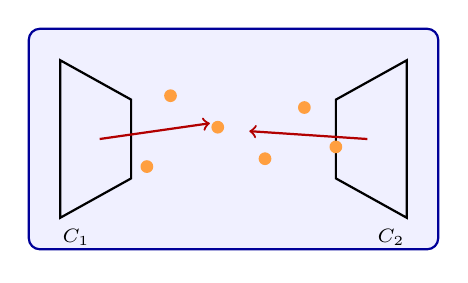
\begin{tikzpicture}[every node/.style={font=\scriptsize}]
\draw[rounded corners, fill=blue!6, draw=blue!60!black, thick] (-2.6,-1.4) rectangle (2.6,1.4);
\draw[thick] (-2.2,-1.0) -- (-1.3,-0.5) -- (-1.3,0.5) -- (-2.2,1.0) -- cycle;
\node at (-2.0,-1.25) {$C_1$};
\draw[thick] (2.2,-1.0) -- (1.3,-0.5) -- (1.3,0.5) -- (2.2,1.0) -- cycle;
\node at (2.0,-1.25) {$C_2$};
\draw[red!70!black, thick, ->] (-1.7,0) -- (-0.3,0.2);
\draw[red!70!black, thick, ->] (1.7,0) -- (0.2,0.1);
\foreach \x/\y in {-0.2/0.15,0.4/-0.25,0.9/0.4,1.3/-0.1,-0.8/0.55,-1.1/-0.35}{
  \fill[orange!75] (\x,\y) circle (2.3pt);
}
\end{tikzpicture}
}

{\scriptsize (a) NeRF: trường liên tục, lấy mẫu theo tia và tích phân thể tích.}
\end{minipage}
\hfill
\begin{minipage}[t]{0.47\textwidth}
\centering
\resizebox{0.92\linewidth}{!}{%
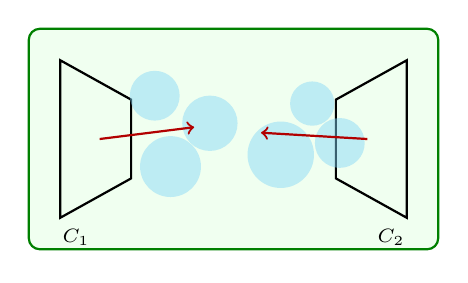
\begin{tikzpicture}[every node/.style={font=\scriptsize}]
\draw[rounded corners, fill=green!6, draw=green!50!black, thick] (-2.6,-1.4) rectangle (2.6,1.4);
\draw[thick] (-2.2,-1.0) -- (-1.3,-0.5) -- (-1.3,0.5) -- (-2.2,1.0) -- cycle;
\node at (-2.0,-1.25) {$C_1$};
\draw[thick] (2.2,-1.0) -- (1.3,-0.5) -- (1.3,0.5) -- (2.2,1.0) -- cycle;
\node at (2.0,-1.25) {$C_2$};
\foreach \x/\y/\r in {-0.3/0.2/10,0.6/-0.2/12,1.0/0.45/8,-1.0/0.55/9,-0.8/-0.35/11,1.35/-0.05/9}{
  \fill[cyan!50, opacity=0.45] (\x,\y) circle (\r pt);
}
\draw[red!70!black, thick, ->] (-1.7,0) -- (-0.5,0.15);
\draw[red!70!black, thick, ->] (1.7,0) -- (0.35,0.08);
\end{tikzpicture}
}

{\scriptsize (b) Gaussian Splatting: dùng các primitive Gaussian explicit để render nhanh hơn.}
\end{minipage}
\caption{Minh họa khái niệm cho hai họ phương pháp scene representation. NeRF biểu diễn scene dưới dạng trường liên tục cần tích phân theo tia nhìn, trong khi Gaussian Splatting dùng các primitive explicit giúp render nhanh hơn.}
\label{fig:nerf-vs-gs}
\end{figure}

\section{Uncertainty, confidence và selective processing}

Trong rất nhiều bài toán dense geometry, confidence và uncertainty đóng vai trò then chốt để kiểm soát chất lượng tái tạo. Ý tưởng chung là không phải mọi quan sát đều đáng tin cậy như nhau; do đó, hệ thống cần có cơ chế đánh giá mức rủi ro hoặc độ chắc chắn để quyết định nên cập nhật mô hình ở đâu và mức nào. Đề tài này tiếp nối tinh thần đó, nhưng đưa nó về mức frame-level selection trong một pipeline UAV reconstruction offline.

\section{Khoảng trống nghiên cứu mà đề tài lựa chọn}

Từ các nhánh trên, có thể rút ra ba nhận xét:
\begin{enumerate}[leftmargin=1.5em]
  \item pipeline cổ điển mạnh về hình học nhưng nặng và khó co giãn theo ngân sách tính toán;
  \item pipeline học sâu mới giúp suy luận geometry dễ hơn, nhưng full-pass trên mọi frame vẫn tốn kém;
  \item số lượng công trình tập trung trực tiếp vào \textit{frame-level refinement budget allocation} trong bài toán UAV reconstruction hiện còn ít.
\end{enumerate}

Đề tài vì thế chọn khoảng trống nghiên cứu sau: \textbf{phân bổ chọn lọc ngân sách refine trong tái tạo hình học UAV bằng một thước đo rủi ro frame-level}.

\end{document}
